\documentclass[12pt,a4paper]{article}

\usepackage[T1]{fontenc}
\usepackage[utf8]{inputenc}
%\usepackage[polish]{babel}
\usepackage{lmodern}
\usepackage{amsmath,latexsym,amsthm,amsfonts,epsfig} %amssymb
%\usepackage{pslatex}
\usepackage{graphicx}
\usepackage{color} 
\usepackage{graphicx}
\usepackage{listings}% listing kodu
\usepackage{dcolumn}
\usepackage{fancybox}
\usepackage{float}
%\usepackage{multirow}
\usepackage{enumerate}
\usepackage{appendix}
\usepackage{fancyhdr}
\begin{document}
\title{\textrm{Pracownia Dyplomowa Magisterska I} \\\mbox{}\\ \textsc{Optimization of Communication Protocols in terms of Data Transfer between FPGA devices and Embedded Systems} \\\mbox{} \\ \textrm{Sprawozdanie}}
\author{Paweł Szostek \\
\texttt{p.szostek@stud.elka.pw.edu.pl}
}
\date{\today}
\maketitle
\section{Introduction}
The aim of the thesis is to design a communication protocol suitable for a transmission in large acquistition systems. The desired protocol must be able to ensure reliable data transfer between FPGAs (Field Programable Gate Arrays) and ARM-based Embedded System (abbreviated as ES) running a distribution of Linux, whereas many FPGA devices may be connected to a single ES over an unreliable network.

The implementation at the FPGA-side must be possibly lightweight and efficient, both in terms of utilization of logic utilization at the FPGA chips as well as with respect to achieving transfer and success rates near the respective maxima. To this end, a two-dimensional (hardware usage-transfer rate) optimization will be done and the design will not require buffering significantly big amounts of data.
The OS-side implementation has to be realized as a Linux Device Driver running in the Kernel mode. This solution will allow to save CPU-time at the package processing by not switching the context from kernel space to user space.

The design will be focused on ensuring the data transfer from FPGAs to ESs. Data flow from ESs to FPGAs will be used for transmision control purposes and not for data transfer itself. 

In parallel to the final driver, there will be implemented a driver interface for testing purposes. It will ease the testing procedure for the FPGA IP core by allowing setting up and controling the communication manually.

The design is planned to be put in Public Domain. This implies not using any closed IP cores, as well as closed pieces of C code in the device driver.
\section{Related work}
\subsection{Available IP cores}
Unfortunatelly, there are not many similar published IP cores available in the internet. Several authors published their hardware descriptions (\cite{Alachiotis11}, \cite{Alachiotis10}, \cite{Zabolotny12}) and this code will be used for deep comparison of the design guidlines and performance. The majority (\cite{Herrmann09}, \cite{Doolittle11}, \cite{Ciobotaru00}, \cite{Lofgren05}) limited their publications to present overall performance results. Searching for available IP cores will be continued later.
\section{Work Plan}
\subsection{Design guidelines}
Designing of the embedded hardware system requires making assumptions regarding simplifaction, parallelization and trade-off between functionality and performance/area. The following issues must be taken into account when designing a protocol targeted for FPGA devices: allowed logic utilization, network speed, number of simultaneous communicating network nodes, packet loss limit.

In order to fulfill requirements for the resource usage for the design there has been made a set of assumptions:
\begin{itemize}
\item the protocol will be held in the Layer 3 (Network Layer) of the ISO/OSI communication stack and will be based on the Ethernet in Layer 2,
\item the protocol will aim to reach full Gigabit Ethernet speed (requiring 125 MHz clock), 
\item the protocol will ensure reliable communication with data integrity between nodes,
\item reliability will be assured by engaging a simple control flow mechanism based on immediate acknowledgement messages sent after receivinge a valid package,
\item data integrity will be based on a checksum mechanism 
\item communication between nodes will be held in a separate private network. This will allow not to implement all remaining L3 protocols, such as ARP or ICMP,
\item solely communication between FPGAs and ESs will be possible. There will not be provided any mechanism for data transfer between FGPAs
\item the design will use an external Gigabit Ethernet PHY (Physical Layer Device), as well as a possibly modified MAC (Layer 2) implementation,
\item frames of up to 1518 bytes will be supported (no support for Ethernet Jumbo frames),
\item the software interface will hide the complexity of setting up the PC-FPGA connection
\end{itemize}
                \begin{figure}[h!]
                \begin{center}
                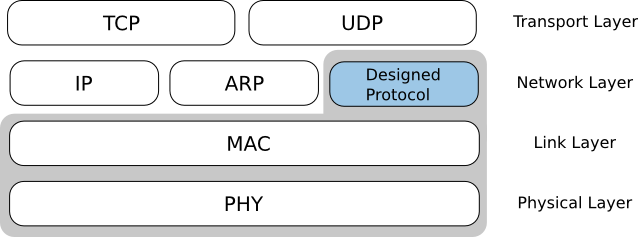
\includegraphics[width=0.65\textwidth]{osi.png}
                \caption{ISO/OSI layers' overview}
                \end{center}
                \end{figure}
                \begin{figure}[h!]
                \begin{center}
                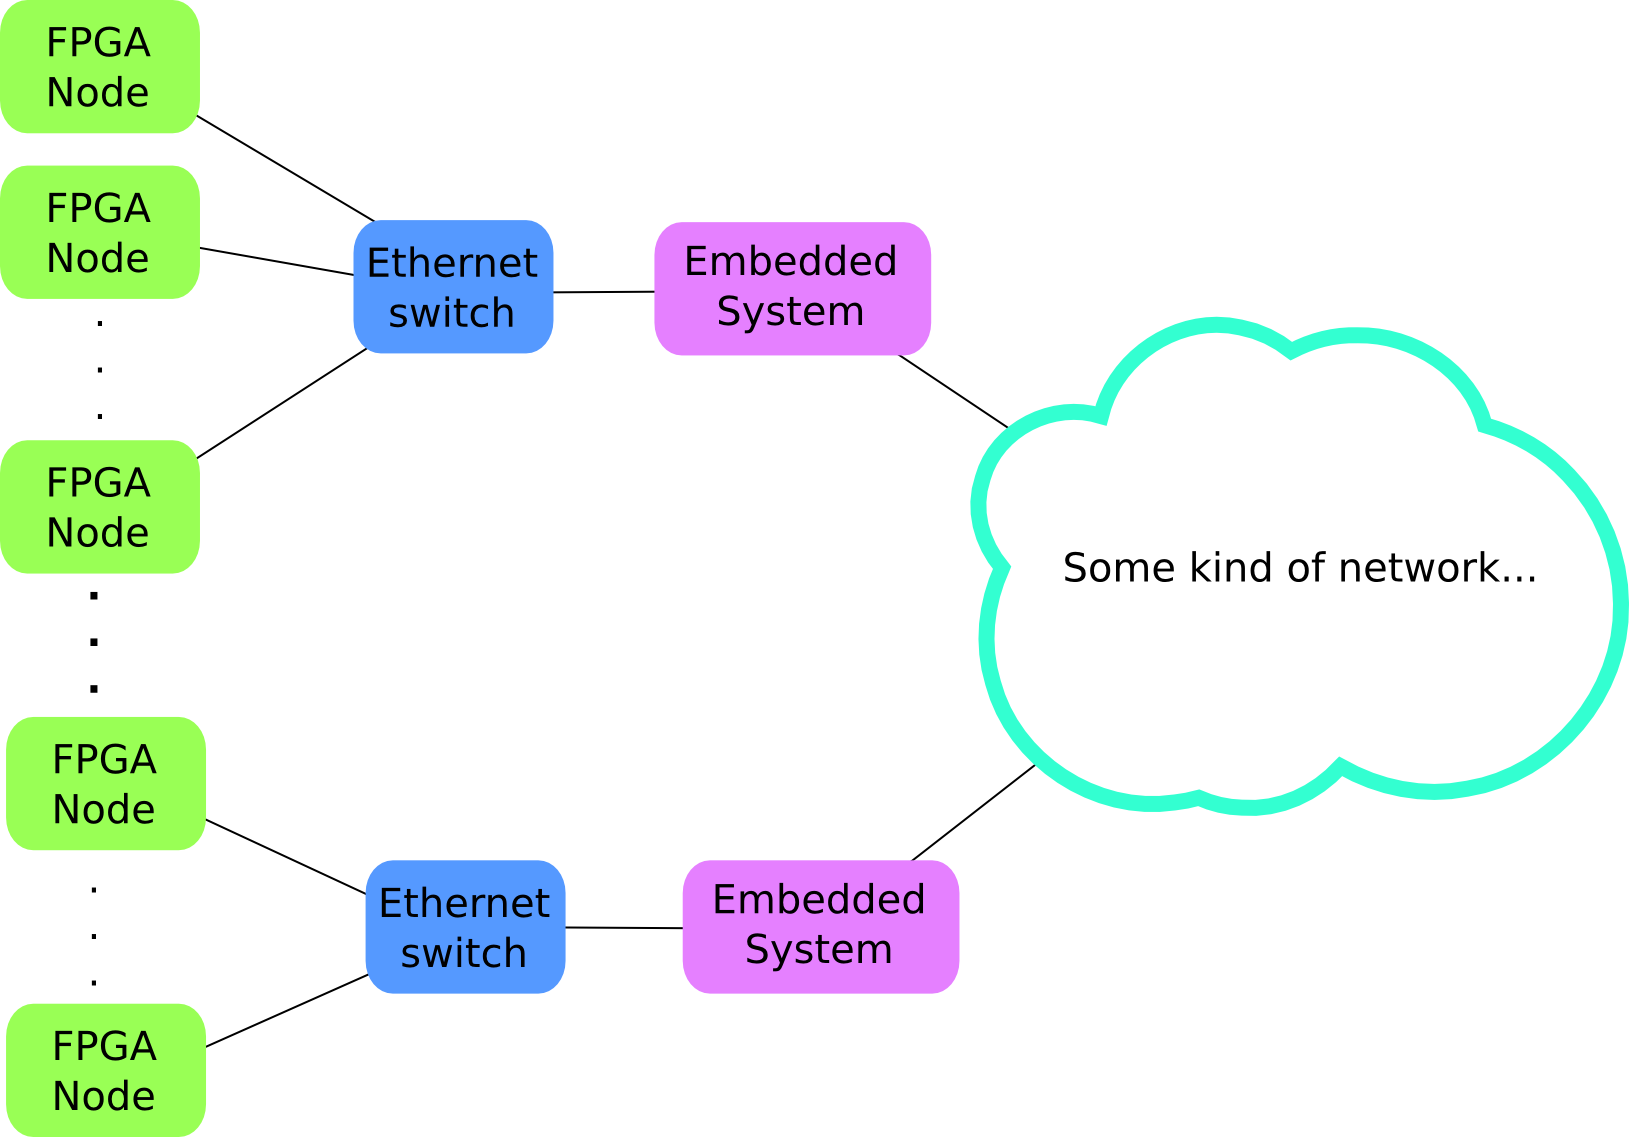
\includegraphics[width=0.75\textwidth]{setup.png}
                \caption{System setup overview}
                \end{center}
                \end{figure}
\subsection{Work packages}
A rough order of the work packages is presented below:
\begin{enumerate}
\item Design of the protocol, description of the forseen use cases,
\item Design of the test framework involving user space device driver,
\item \{Implementation - Performance test - Optimization\} loop,
\item Test with several nodes connected to a PC via an ethernet switch,
\item Implementation of a proper kernel space device driver,
\item Tests in the target setup.
\end{enumerate}
Content of each package will be extended before starting the design phase and will be further precised. 

\subsection{Optimizations planned}
One of the main issues concerning resource usage at the FPGA chip is buffering space needed by the protocol. In cases when it is required to use internal RAM only we are limited, generally speaking, to a very limited amount of space. This means that in order to keep transmission fluent and to be able to continuously receive new. 

Let's take Xilinx Spartan 3 XC3S1000 chip as example. It offers 432k bits of of Block RAM which is equal to 54kB of memory.
When designing the protocol one must keep in mind that the reason for packet losses might be the data transfer itself. If packets are too massively to the Embedded System it might be not able to serve all of them 

Opposed to many existing solutions, I will not implement an optimized UPD/IP stack. The main requirement for the system is to provide reliable communication and this would involve building another protocol above or parallel to UDP. Nevertheless, I will certainly make use of optimizations proposed in the analyzed literature: 

\subsection{Tests}
The final design will be verified using a Virtex 5 evaluation board(s). The IP core will be compared to other available designs presented in \cite{Lofgren05}, \cite{Alachiotis10}, \cite{Alachiotis11}, \cite{Herrmann09} and \cite{Zabolotny12}. It must be mentioned that the source of designs described in \cite{Herrmann09} and \cite{Lofgren05} are put in the public domain. For this reason a direct comparison will not be able and a comparison based on logic slices usage and clock speed will be done.
\mbox{}
First part of testing will be focused on a single IP Core placed on an FPGA connected to a PC. The driver will be implemented as a user space program and will 

\renewcommand{\refname}{Analyzed literature}
\begin{thebibliography}{99}
\bibitem{Lofgren05}P
L\"ofgren A., Lodesten L., Sj\"oholm S., Hansson H.: \emph{An analysis of FPGA-based UDP/IP stack parallelism for embedded Ethernet connectivity},
Proceedings of NORCHIP 2005, pp. 94-97.
\bibitem{Alachiotis11}
Alachiotis N., Berger S., Stamatakis A.: \emph{A Versatile UDP/IP based PC - FPGA Communication Platform},
Open Access at Open Cores.
\bibitem{Alachiotis10}
Alachiotis N., Berger S., Stamatakis A.: \emph{Efficient PC-FPGA communication over Gigabit Ethernet},
Open Access at Open Cores.
\bibitem{Tsakiris07}
Tsakiris N., Knowles G.: \emph{A Gigabit IP Core for Embedded Systems},
International Journal of Circuits, Systems and Signal Processing, 2007, pp. 347-355.
\bibitem{Herrmann09}
Herrmann F., Perin G., de Freitas J., Bertagnolli R., dos Santos Martins J.: \emph{A Gigabit UDP/IP Network Stack in FPGA},
Proceedings of 16th International Conference on Electronics, Circuits and Systems, 2009, pp. 836-839.
\bibitem{Moohsenin04}
Mohsenin T.: \emph{Design and Evaluation of FPGA-Based Gigabit-Ethernet/PCI Network Interface Card},
Master Thesis at the University of Texas, 2004.
\bibitem{Kachris01}
Kachris C.: \emph{Design and Implementation of a TCP/IP core for reconfigurable logic},
Master Thesis at the Techical University of Crete, 2001.
\bibitem{Lu03}
Lu W.: \emph{Designing TCP/IP Functions In FPGAs},
Master Thesis at the Delft University of Technology, 2003.
\bibitem{Kuhn07}
Kuhn w. et al.: \emph{FPGA based Compute Nodes for High Level Triggering in PANDA},
Proceedings of International Conference on Computing in High Energy and Nuclear Physics CHEP'07.
\bibitem{Doolittle11}
Doolittle L., Serrano C.: \emph{FPGA Communication based on Gigabit Ethernet},
Proceedings of ICALEPCS 2011.
\bibitem{Ciobotaru00}
Ciobotaru M., Ivanovici M., Beuran R., Stancu S.: \emph{Versatile FPGA-based Hardware Platform for Gigabit Ethernet Applications},
6th Annual Postgraduate Symposium, Liverpool, U.K., 2005, pp. 391-395.
\bibitem{Yusta00}
Yusta J., Zenor J., Kredo II K.: \emph{Efficient High-Speed Ethernet for Real Time Simulation},
Proceedings of ISMC 2011.
\bibitem{Zabolotny12}
Zabołotny W.: \emph{Layer 3 ethernet protocol for FPGA based systems}, 
\emph{http://www.ise.pw.edu.pl/\~{}wzab/fpga\_l3\_fade/}, 2012.

\end{thebibliography}
\end{document}

